\chapter{Implementasi dan Pengujian}

Pada bab ini, akan dibahas implementasi dari modifikasi pengoptimasi yang sebelumnya telah dibahas, serta perbandingannya dengan penelitian dari \textcite{Chen2022Efficient} dan \textcite{Chen2021CADA}.

\section{Implementasi}
Algoritma pengoptimasi yang dijelaskan dalam penelitian \textcite{Chen2022Efficient} dan \textcite{Chen2021CADA} masing-masing akan diimplementasikan menggunakan pustaka PyTorch dengan arsitektur \emph{parameter server}. Kemudian, implementasi modifikasi penggabungan akan didasarkan kepada hasil implementasi kedua pengoptimasi.

Setiap pengoptimasi akan dibagi menjadi tiga bagian, yakni \emph{parameter server}, \emph{trainer}, dan \emph{runner}. Bagian \emph{parameter server} memiliki tugas umum menjadi \emph{node} yang menyimpan model utama. Kemudian, \emph{trainer} akan mendapatkan parameter model dari \emph{parameter server} dan melakukan perhitungan gradien. Gradien yang telah dihitung lalu dikirim kembali kepada \emph{parameter server} untuk memperbarui parameter model. Bagian yang akan mengorkestrasi hubungan ini adalah \emph{runner}.

Algoritma untuk pengoptimasi gabungan akan dibagi menjadi 2, yakni bagian \textit{parameter server} serta bagian \textit{worker}. Algoritma untuk \textit{parameter server} dapat dilihat pada algoritma~\ref{myadam_server}. Algoritma untuk \textit{worker} dapat dilihat pada algoritma~\ref{myadam_worker}. Kondisi yang digunakan untuk menentukan pengiriman dari tiap \textit{worker} dapat dilihat pada pertaksamaan~\ref{cada2cond}.

\begin{equation}
  \label{cada2cond}
  \|\nabla f_t(\theta_t) - \nabla f_t(\theta_{t-\tau})\|^2 \leq \frac{c}{D} \sum_{d=1}^{D} \|\theta_{t+1-d} - \theta_{t-d}\|^2
\end{equation}

\begin{algorithm}[H]
  \setstretch{1}
  \caption{Modifikasi Adam untuk Parameter Server}\label{myadam_server}
  \begin{algorithmic}[1]
    \State \textbf{Parameter:} Fungsi Kuantisasi $\mathcal{Q}_s$
    \State \textbf{Inisialisasi} vektor parameter $\theta_0$, error term $e_1 \gets 0$
    \State Sebarkan $\theta_0$ ke semua \textit{worker}
    \For{$t = 1,2,\dots,T$}
    \State $\hat{\delta_t} \gets \textnormal{rata-rata } \delta_t^{(i)}$ dari setiap \textit{worker}
    \State Sebarkan $\tilde{\delta_t} \gets \mathcal{Q}(\hat{\delta_t} + e_t)$
    \State $e_{t+1} \gets e_{t}$
    \State $\theta_{t+1} \gets \theta_t - \tilde{\delta_t}$
    \EndFor
  \end{algorithmic}
\end{algorithm}

\begin{algorithm}[H]
  \caption{Modifikasi Adam untuk Worker ke-$i$}\label{myadam_worker}
  \setstretch{1}
  \begin{algorithmic}[1]
    \State \textbf{Parameter:} Fungsi Kuantisasi $\mathcal{Q}_w$, Hyperparameter Adam $\alpha, \beta_1, \beta_2$, konstanta batas $c$, batas maksimum penundaan $D$
    \State $m_0^{(i)} \gets 0, v_0^{(i)} \gets \epsilon, e_1^{(i)} \gets 0, \tau^{(i)} \gets 0$
    \State $\theta^{(i)}_0 \gets \theta_1$ dari server
    \For{$t=1,2,\dots,T$}
    \State $g_t^{(i)} \gets \nabla_\theta f_t(\theta_{t})$
    \State $v_t^{(i)} \gets \theta_t v_{t-1}^{(i)} + (1-\theta_t)[g_t^{(i)}]^2$
    \State $m_t^{(i)} \gets \beta_1 m_{t-1}^{(i)} + (1-\beta_1)g_t^{(i)}$
    \State $\alpha_t \gets \alpha \sqrt{1-\beta_2^t}/(1-\beta_1^t)$
    \State $\delta^{(i)} \gets \alpha_t m_t^{(i)}/\sqrt{v_t^{(i)}}+e_t^{(i)}$
    \State $\theta_t \gets \theta_{t-1} - \delta^{(i)}$
    \State Hitung $\nabla f_t(\theta^{(i)}_{t})$ dan $\nabla f_t(\theta^{(i)}_{t-\tau})$
    \State $\delta^{(i)} \gets \mathcal{Q}_w(\delta^{(i)})$
    \If{Kondisi \ref{cada2cond} tidak terpenuhi atau $\tau \ge D$}
    \State Kirim $\delta^{(i)}$
    \State $\tau \gets 1$
    \Else
    \State $\tau \gets \tau + 1$
    \EndIf
    \State $e_{t+1}^{(i)} \gets \alpha_t \frac{m_t^{(i)}}{\sqrt{v_t^{(i)}}} + e_t^{(i)} - \delta_t^{(i)}$
    \State Terima $\tilde{\delta_t}$ dari server
    \State $\theta_{t} \gets \theta_{t-1} - \tilde{\delta_t}$
    \EndFor
  \end{algorithmic}
\end{algorithm}

\section{Pengujian}
\subsection{Lingkungan Pengujian}
Pengujian dilakuan pada server DGX dengan spesifikasi pada tabel~\ref{dgx}. Namun, pengujian dilakukan dengan melakukan simulasi \emph{deep learning} terdistribusi pada hanya satu GPU.

\begin{table}[H]
  \caption{Spesifikasi Lingkungan Pengujian}\label{dgx}
  \centering
  \setstretch{1.5}
  \begin{tabular}{ | c | c | }
    \hline
    \textbf{Parameter} & \textbf{Spesifikasi}                           \\
    \hline
    CPU                & 2x Intel Xeon E5-2698 v3 (16-core, Haswell-EP) \\
    \hline
    RAM                & 512GB DDR4-2133                                \\
    \hline
    GPU                & 8x Tesla V100 32GB VRAM                        \\
    \hline
    Penyimpanan        & 4x1.92 TB SSD                                  \\
    \hline
  \end{tabular}
\end{table}

Selain itu, versi perangkat lunak dan pustaka dapat dilihat pada tabel~\ref{softwares}.
\begin{table}[H]
  \caption{Versi Perangkat Lunak}\label{softwares}
  \centering
  \setstretch{1.5}
  \begin{tabular}{ | c | c | }
    \hline
    \textbf{Perangkat Lunak} & \textbf{Versi} \\
    \hline
    Python                   & 3              \\
    \hline
    PyTorch                  & 1.13.1+cuda    \\
    \hline
    TorchVision              & 0.14.1+cuda    \\
    \hline
  \end{tabular}
\end{table}

\subsection{Skenario Pengujian}
Terdapat dua skenario pelatihan model \emph{deep learning} yang akan dilakukan untuk menguji teknik yang diimplementasi. Dalam skenario pertama, akan dilatih sebuah model sederhana untuk melakukan klasifikasi terhadap \emph{dataset} Fashion-MNIST \parencite{xiao2017fashion}. Kemudian, dalam skenario kedua, akan dilatih model ResNet-20 \parencite{he2015deep} untuk melakukan klasifikasi terhadap \emph{dataset} CIFAR-10 \parencite{krizhevsky2009cifar}.

\emph{Dataset} Fashion-MNIST merupakan dataset yang berisi gambar pakaian dari Zalando, dengan 60.000 data untuk pelatihan dan 10.000 data untuk pengujian \parencite{xiao2017fashion}. Setiap data merupakan gambar berukuran 28 $\times$ 28 piksel yang dikategorikan ke dalam 10 kelas.

\emph{Dataset} CIFAR-10 merupakan dataset yang berisi 60.000 gambar berwarna berukuran 32 $\times$ 32 piksel. Gambar-gambar tersebut dikategorikan ke dalam 10 kelas, dengan setiap kelas berisi 60.000 gambar. \emph{Dataset} tersebut dibagi menjadi 50.000 data untuk pelatihan dan 10.000 data untuk pengujian.

Dalam kedua skenario, \emph{dataset} disebarkan ke 10 \emph{trainer} yang masing-masing dijalankan pada proses berbeda. Komunikasi antar proses dilakukan dengan bantuan modul RPC pada pustaka PyTorch. Kemudian, pelatihan dilakukan menggunakan GPU yang terdapat pada lingkungan pengujian. Seluruh worker dialokasikan pada GPU yang sama, namun masing-masing worker memiliki salinan model yang terpisah satu sama lain.

Pengujian dilakukan dengan merekam jumlah byte yang dipertukarkan serta jumlah komunikasi yang dilakukan antara \emph{parameter server} dengan \emph{trainer}. Selain itu, akurasi dan nilai \emph{loss} setiap \emph{epoch} akan direkam untuk membandingkan hasil model. Pengujian dilakukan untuk masing-masing teknik secara terpisah menggunakan \emph{hyperparameter} yang ditentukan.

Jumlah komunikasi yang direkam dalam pengujian adalah semua komunikasi yang dilakukan dari dan ke \emph{parameter server}. Dalam teknik CADA, komunikasi berarti pendistribusian model kepada setiap \emph{trainer} serta pengiriman gradien dari tiap worker ke \emph{parameter server}, bila ada. Dalam teknik Efficient-Adam, komunikasi berarti pendistribusian model saat pertama kali dijalankan, serta pengiriman perubahan parameter dari setiap \emph{trainer} ke \emph{parameter server} dan pendistribusian perubahan parameter dari \emph{parameter server} ke setiap \emph{trainer}.

Perhitungan jumlah byte yang digunakan untuk komunikasi dilakukan dengan cara mengalikan jumlah elemen dari setiap tensor yang dikirimkan dengan jumlah byte yang diperlukan untuk menyimpan satu buah elemen dengan tipe dari tensor tersebut. Sebagai contoh, sebuah tensor bertipe float32 dengan 8 elemen akan menggunakan 32 byte, karena sebuah elemen dengan tipe data float32 membutuhkan 4 byte untuk penyimpanan.

Pemilihan \emph{hyperparameter} dilakukan secara terpisah untuk kedua skenario, dan untuk setiap teknik. Namun, \emph{learning rate} akan berkurang seiring bertambahnya epoch. Setiap epoch tertentu, \emph{learning rate} yang digunakan akan berkurang sebanyak setengah \emph{learning rate} saat itu. Untuk kedua skenario, pengurangan dilakukan setiap 100 epoch.

Model yang digunakan untuk mengklasifikasi Fashion-MNIST adalah sebuah model dengan dua buah \emph{layer} konvolusi yang memiliki fungsi aktivasi ELU dan operasi \emph{max pooling}, diikuti oleh sebuah \emph{layer} yang terhubung penuh untuk membuat prediksi. Arsitektur model yang dibangun dapat dilihat pada gambar~\ref{fashionmnist}. Model tersebut memiliki parameter sejumlah 24.778 yang terbagi dalam 7 \emph{layer}.

\begin{figure}
  \centering
  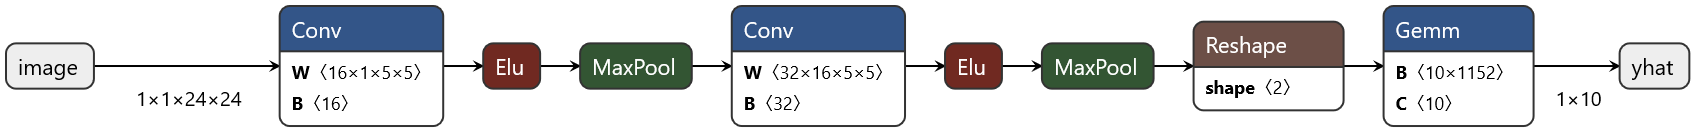
\includegraphics[width=\textwidth]{fashion_mnist.onnx.png}
  \caption{Arsitektur model sederhana untuk klasifikasi Fashion-MNIST}\label{fashionmnist}
\end{figure}

Pemilihan \emph{hyperparameter} untuk model tersebut dapat dilihat pada tabel~\ref{hyperparamfashion}. Fungsi kuantisasi yang digunakan untuk teknik Efficient-Adam serta teknik gabungan adalah pemetaan langsung ke tipe data \emph{float16} pada PyTorch. Ukuran \emph{minibatch} yang digunakan dalam pembelajaran adalah 60.

\begin{table}[H]
  \caption{Pemilihan \emph{Hyperparameter} untuk klasifikasi Fashion-MNIST}\label{hyperparamfashion}
  \centering
  \setstretch{1.5}
  \begin{tabular}{ | c | c | c | }
    \hline
    \textbf{Teknik}                                               & \textbf{Parameter} & \textbf{Nilai} \\
    \hline
    \multirow{5}{*}{CADA, \textcite{Chen2021CADA}}                & $\alpha$           & 0.00001        \\
                                                                  & $\beta_1$          & 0.9            \\
                                                                  & $\beta_2$          & 0.99           \\
                                                                  & $D$                & 50             \\
                                                                  & $d_{max}$          & 10             \\
                                                                  & $c$                & 400            \\
    \hline
    \multirow{3}{*}{Efficient-Adam, \textcite{Chen2022Efficient}} & $\alpha$           & 0.0001         \\
                                                                  & $\beta_1$          & 0.9            \\
                                                                  & $\beta_2$          & 0.999          \\
    \hline
    \multirow{5}{*}{Gabungan}                                     & $\alpha$           & 0.0001         \\
                                                                  & $\beta_1$          & 0.9            \\
                                                                  & $\beta_2$          & 0.99           \\
                                                                  & $D$                & 50             \\
                                                                  & $d_{max}$          & 10             \\
                                                                  & $c$                & 400            \\
    \hline
  \end{tabular}
\end{table}


Model yang digunakan untuk mengklasifikasi \emph{dataset} CIFAR-10 adalah ResNet-20. Model ResNet-20, atau secara umum ResNet, merupakan model yang menggunakan pemetaan residu $\mathcal{H}(x) = \mathcal{F}(x) + x$ \parencite{he2015deep}, yang memberikan prekondisi pemetaan identitas untuk model. Menurut eksperimen yang dilakukan \textcite{he2015deep}, pemetaan identitas merupakan prekondisi yang cukup masuk akal. pemetaan residu dapat dibuat sebagai sebuah hubungan langsung dari titik tertentu ke titik lain, melompati beberapa \emph{layer}. Ilustrasi dari sebuah blok residu dapat dilihat pada gambar~\ref{resblock}.

\begin{figure}[htb]
  \centering
  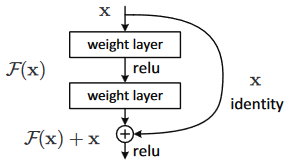
\includegraphics[width=0.5\textwidth]{resblock.png}
  \caption{Ilustrasi sebuah blok residu \parencite{he2015deep}}\label{resblock}
\end{figure}

Model ResNet-20 yang digunakan dalam pengujian diambil dari \emph{repository} GitHub \cite{Idelbayev18a} dengan beberapa perubahan agar dapat digunakan pada CPU dan GPU. Model tersebut memiliki jumlah parameter sebanyak 0.27 juta dalam 20 \emph{layer}.

Pemilihan \emph{hyperparameter} untuk masing-masing teknik dapat dilihat pada tabel~\ref{hyperparamresnet}. Fungsi kuantisasi yang digunakan sama seperti skenario sebelumnya, yakni menggunakan pemetaan langsung ke tipe data \emph{float16} pada PyTorch.

\begin{table}[H]
  \caption{Pemilihan \emph{Hyperparameter} untuk klasifikasi CIFAR-10}\label{hyperparamresnet}
  \centering
  \setstretch{1.5}
  \begin{tabular}{ | c | c | c | }
    \hline
    \textbf{Teknik}                                               & \textbf{Parameter} & \textbf{Nilai} \\
    \hline
    \multirow{5}{*}{CADA, \textcite{Chen2021CADA}}                & $\alpha$           & 0.01           \\
                                                                  & $\beta_1$          & 0.9            \\
                                                                  & $\beta_2$          & 0.99           \\
                                                                  & $D$                & 50             \\
                                                                  & $d_{max}$          & 2              \\
                                                                  & $c$                & 0.12           \\
    \hline
    \multirow{3}{*}{Efficient-Adam, \textcite{Chen2022Efficient}} & $\alpha$           & 0.0005         \\
                                                                  & $\beta_1$          & 0.9            \\
                                                                  & $\beta_2$          & 0.999          \\
    \hline
    \multirow{5}{*}{Gabungan}                                     & $\alpha$           & 0.0005         \\
                                                                  & $\beta_1$          & 0.9            \\
                                                                  & $\beta_2$          & 0.999          \\
                                                                  & $D$                & 50             \\
                                                                  & $d_{max}$          & 2              \\
                                                                  & $c$                & 0.12           \\
    \hline
  \end{tabular}
\end{table}

\subsection{Hasil Pengujian}

Hasil yang akan dibandingkan dalam kedua skenario adalah jumlah komunikasi serta jumlah byte yang digunakan untuk komunikasi. Akurasi deri setiap model juga akan dibandingkan untuk mengevaluasi model akhir yang dihasilkan.

\subsubsection{\emph{Dataset} Fashion-MNIST}

Plot akurasi tiap epoch untuk ketiga teknik dapat dilihat pada gambar~\ref{fashion_acc}. Dalam plot tersebut dapat dilihat akurasi model yang dihasilkan teknik Efficient-Adam serta teknik gabungan berada di sekitar 84 hingga 86 persen. Dibandingkan kedua teknik tersebt, teknik CADA hanya menghasilkan model yang memiliki akurasi sekitar 70 persen.

\begin{figure}[H]
  \centering
  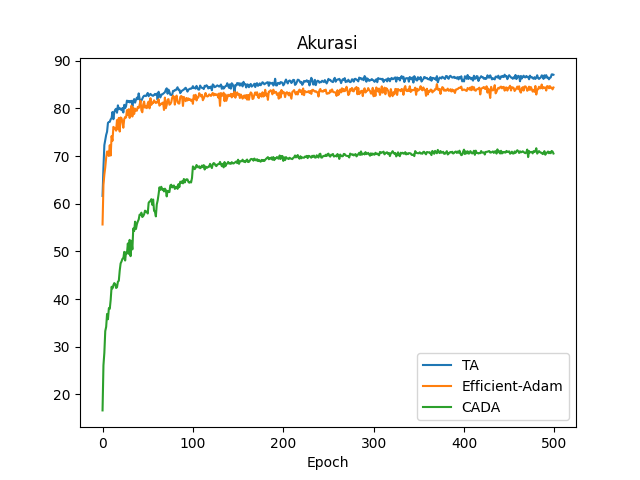
\includegraphics[width=\textwidth]{fashion_acc.png}
  \caption{Akurasi tiap teknik dalam pelatihan pada Fashion-MNIST}\label{fashion_acc}
\end{figure}

Plot perbandingan jumlah komunikasi per epoch untuk tiap teknik dapat dilihat pada gambar~\ref{fashion_comms}. Teknik CADA menggunakan 1000 komunikasi per epoch, tanpa ada pengurangan sama sekali. Teknik gabungan juga tidak mampu mengurangi jumlah komunikasi sama sekali, dengan jumlah komunikasi yang sama dengan teknik CADA.

\begin{figure}[H]
  \centering
  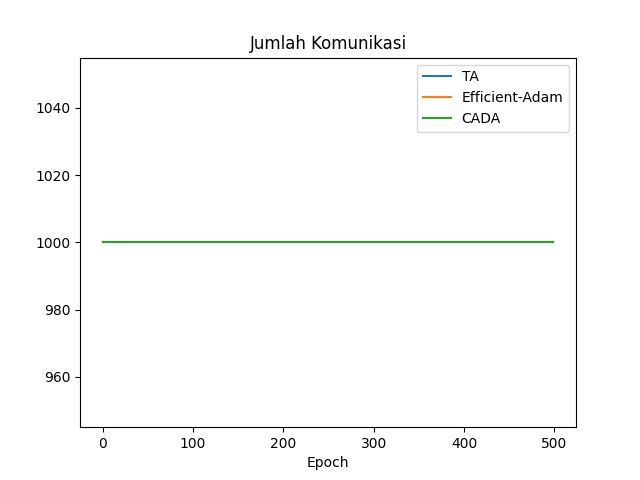
\includegraphics[width=\textwidth]{fashion_comms.png}
  \caption{Jumlah komunikasi tiap teknik dalam pelatihan pada Fashion-MNIST}\label{fashion_comms}
\end{figure}

Plot perbandingan jumlah byte yang digunakan dapat dilihat pada gambar~\ref{fashion_bits}. Jumlah byte yang paling sedikit digunakan adalah pada teknik Efficient-Adam, yang menggunakan 0.92 kali teknik gabungan. Teknik gabungan menggunakan lebih banyak byte untuk berkomunikasi karena adanya kebutuhan untuk mendistribusikan nilai ambang pada pertaksamaan~\ref{cada2cond}.

\begin{figure}[H]
  \centering
  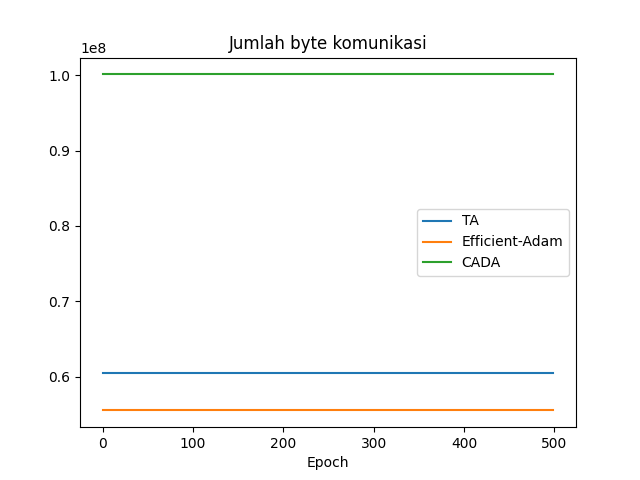
\includegraphics[width=\textwidth]{fashion_bits.png}
  \caption{Jumlah byte tiap teknik dalam pelatihan pada Fashion-MNIST}\label{fashion_bits}
\end{figure}


\subsubsection{\emph{Dataset} CIFAR-10}

Plot akurasi tiap epoch untuk ketiga teknik dapat dilihat pada gambar~\ref{resnet_acc}. Dalam plot tersebut dapat dilihat akurasi model yang dihasilkan ketiga teknik berada di atas 80\%, dengan Efficient-Adam terletak sedikit lebih di atas kedua teknik lainnya.

\begin{figure}[H]
  \centering
  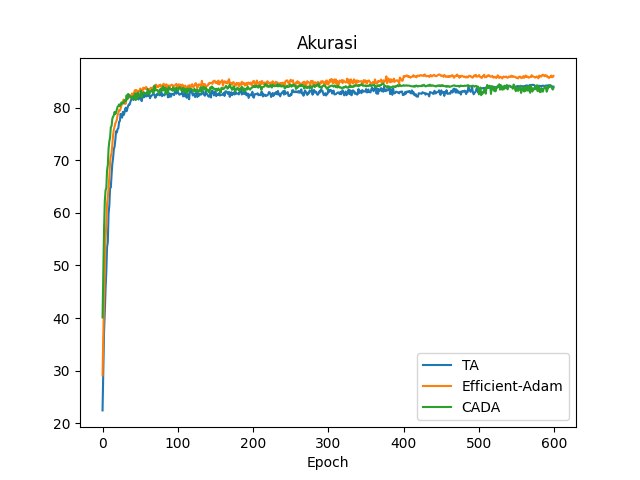
\includegraphics[width=\textwidth]{resnet_acc.png}
  \caption{Akurasi tiap teknik dalam pelatihan ResNet-20}\label{resnet_acc}
\end{figure}

Plot perbandingan jumlah komunikasi per epoch untuk tiap teknik dapat dilihat pada gambar~\ref{resnet_comms}. Dalam plot tersebut, terlihat bahwa teknik Efficient-Adam sangat berimpitan dengan CADA. Namun, teknik CADA mampu mengurangi sedikit jumlah komunikasi. Di sisi lain, implementasi gabungan memberikan pengurangan jumlah komunikasi yang cukup banyak, hingga hanya membutuhkan kurang dari 825 komunikasi di sebelum epoch 600.

\begin{figure}[H]
  \centering
  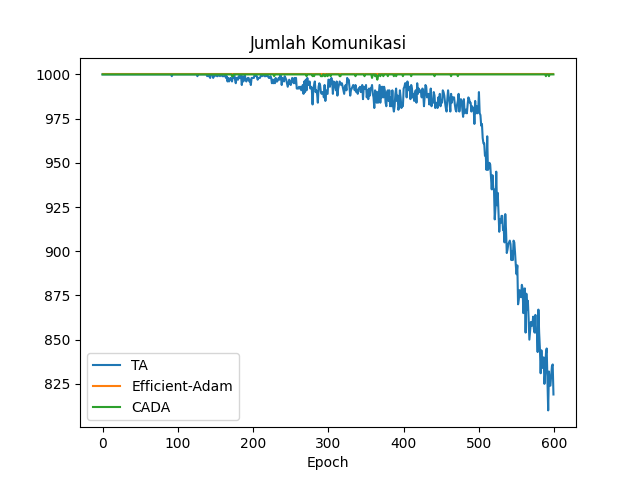
\includegraphics[width=\textwidth]{resnet_comms.png}
  \caption{Jumlah komunikasi tiap teknik dalam pelatihan ResNet-20}\label{resnet_comms}
\end{figure}

Plot perbandingan jumlah byte yang digunakan dapat dilihat pada gambar~\ref{resnet_bits}. Dapat dilihat bahwa jumlah byte yang digunakan oleh CADA sekitar 4 kali lebih besar dibandingkan Efficient-Adam serta teknik gabungan. Namun, terlihat bahwa teknik gabungan menggunakan lebih banyak byte dibandingkan Efficient-Adam. Kemudian, jumlah byte yang digunakan oleh teknik gabungan terlihat berkurang sesuai dengan pengurangan jumlah komunikasi yang terjadi.

\begin{figure}[H]
  \centering
  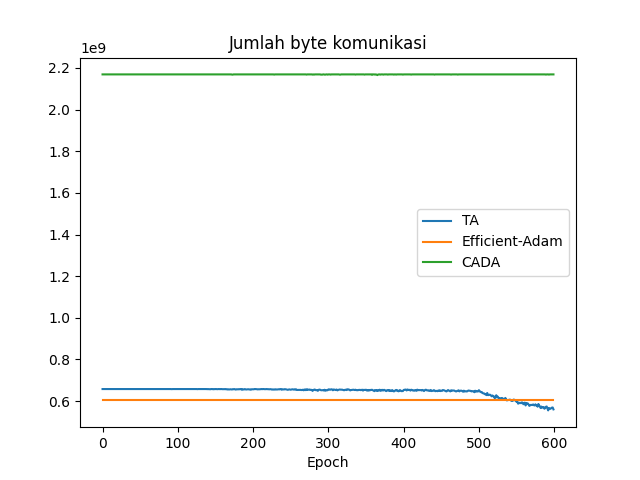
\includegraphics[width=\textwidth]{resnet_bits.png}
  \caption{Jumlah byte tiap teknik dalam pelatihan ResNet-20}\label{resnet_bits}
\end{figure}


\subsection{Analisis Hasil Pengujian}

Berdasarkan pengujian yang dilakukan dalam kedua skenario, didapatkan bahwa teknik gabungan dapat menggunakan jumlah byte lebih sedikit dibandingkan CADA. Bahkan, teknik gabungan mampu mengurangi jumlah komunikasi dalam skenario pelatihan model yang lebih kompleks yakni ResNet-20. Namun, teknik gabungan tetap membutuhkan sedikit lebih banyak byte untuk melakukan komunikasi dibandingkan Efficient-Adam. Penyebab lebih banyaknya jumlah byte adalah adanya nilai tambahan yang perlu dikomunikasikan oleh \emph{parameter server}, yakni nilai ambang yang digunakan dalam pertaksamaan~\ref{cada2cond}.

Pengurangan jumlah komunikasi pada skenario \emph{dataset} CIFAR-10 lebih baik dibandingkan pada skenario \emph{dataset} Fashion-MNIST. Dalam skenario \emph{dataset} CIFAR-10, model ResNet-20 memiliki jumlah parameter yang banyak, sehingga nilai ambang yang dihitung akan lebih besar. Di sisi lain, model sederhana yang digunakan dalam skenario \emph{dataset} Fashion-MNIST memiliki jumlah parameter jauh lebih sedikit, sehingga nilai ambang yang didapatkan lebih kecil. Oleh karena itu, lebih mudah untuk mencapai nilai ambang pada skenario \emph{dataset} Fashion-MNIST.

Kemudian, jumlah komunikasi yang dilakukan oleh CADA juga masih tidak berkurang sebanyak jumlah komunikasi dalam teknik gabungan. Hal ini mungkin disebabkan karena \emph{hyperparameter} yang dipilih menyebabkan nilai selisih gradien yang didapatkan selalu besar. Dampaknya, pertaksamaan~\ref{cada2cond} jarang terpenuhi. Hal tersebut tidak terlihat pada teknik gabungan karena nilai pembaruan dikuantisasi. Hal tersebut menurunkan presisi nilai ambang. Kemudian, perkembangan gradien akan dipengaruhi oleh \emph{error-feedback}, sehingga perkembangan gradien mungkin menjadi lebih kecil.

Pemilihan nilai \emph{hyperparameter} yang berbeda, seperti memilih nilai $\alpha$ yang lebih kecil atau lebih besar menyebabkan model yang dihasilkan memiliki akurasi lebih rendah. Penggunaan nilai $\alpha$ yang terlalu kecil dapat menyebabkan model mencapai minima lokal. Namun, penggunaan nilai $\alpha$ yang terlalu besar juga dapat menghambat proses pelatihan model.

Pemilihan \emph{hyperparameter} $\beta_1$ maupun $\beta_2$ juga dapat memengaruhi kecepatan konvergensi serta akurasi model yang dihasilkan. yang lebih besar dapat membantu dalam pelatihan agar tidak terjebak dalam minima lokal, namun model lebih sulit untuk konvergen karena momentum yang terlalu besar.

Pemilihan nilai $c$ yang digunakan sebagai konstanta dalam pertaksamaan~\ref{cada2cond} memengaruhi jumlah komunikasi yang diperlukan oleh CADA maupun teknik gabungan. Apabila nilai c terlalu besar, maka komunikasi yang dilakukan akan menjadi sedikit sehingga konvergensi model semakin lambat. Namun, apabila nilai c terlalu kecil, maka pengurangan komunikasi akan terjadi lebih jarang.

Pemilihan nilai $D$ serta $d_{max}$ sebagai \emph{hyperparameter} juga dapat memengaruhi jumlah komunikasi yang diperlukan. Akibatnya, konvergensi model juga akan terpengaruh. Pemilihan nilai $D$ akan berpengaruh terhadap komunikasi yang dilakukan oleh \emph{worker} tertentu apabila \emph{worker} tersebut tidak memberikan peningkatan gradien yang besar. Selain itu, nilai $d_{max}$ akan memengaruhi nilai ambang yang dihasilkan. Semakin besar nilai $d_{max}$, maka semakin banyak nilai ambang historis yang akan memengaruhi nilai ambang selanjutnya.
